\section{Date: 2026-11-16}
\noindent \textbf{Series ID: IEAAPIN} 

\noindent This series is titled US Acquisition of Portfolio Investment Assets and has a frequency of Quarterly. The units are Millions of Dollars and the seasonal adjustment is Not Seasonally Adjusted.The observation start date is 1999-01-01 and the observation end date is 2026-04-01.The popularity of this series is 3. \\ 

\noindent \textbf{Series ID: MDOTHMPTFHLMCTP1T4FR} 

\noindent This series is titled Mortgage Debt Outstanding by Type of Holder and Property: Mortgage Pools or Trust: Federal Home Loan Mortgage Corporation for One- to Four-Family Residences (DISCONTINUED) and has a frequency of Quarterly, End of Period. The units are Millions of Dollars and the seasonal adjustment is Not Seasonally Adjusted.The observation start date is 1949-01-01 and the observation end date is 2019-07-01.The popularity of this series is 1. \\ 

\subsection{Raw Regression}
\noindent Regresses the two series against each other directly. A significant result here can come just as easily from both series sharing a long-run trend as from any real relationship.

\begin{center}
\begin{tabular}{lclc}
\toprule
\textbf{Dep. Variable:}       & value\_fred\_MDOTHMPTFHLMCTP1T4FR & \textbf{  R-squared:         } &     0.013   \\
\textbf{Model:}               &                OLS                & \textbf{  Adj. R-squared:    } &     0.001   \\
\textbf{Method:}              &           Least Squares           & \textbf{  F-statistic:       } &     1.053   \\
\textbf{Date:}                &          Mon, 16 Nov 2026         & \textbf{  Prob (F-statistic):} &    0.308    \\
\textbf{Time:}                &              21:19:14             & \textbf{  Log-Likelihood:    } &   -1229.8   \\
\textbf{No. Observations:}    &                   83              & \textbf{  AIC:               } &     2464.   \\
\textbf{Df Residuals:}        &                   81              & \textbf{  BIC:               } &     2468.   \\
\textbf{Df Model:}            &                    1              & \textbf{                     } &             \\
\textbf{Covariance Type:}     &             nonrobust             & \textbf{                     } &             \\
\bottomrule
\end{tabular}
\begin{tabular}{lcccccc}
                              & \textbf{coef} & \textbf{std err} & \textbf{t} & \textbf{P$> |$t$|$} & \textbf{[0.025} & \textbf{0.975]}  \\
\midrule
\textbf{const}                &    7.098e+05  &     9.06e+04     &     7.831  &         0.000        &     5.29e+05    &      8.9e+05     \\
\textbf{value\_fred\_IEAAPIN} &      -0.9739  &        0.949     &    -1.026  &         0.308        &       -2.862    &        0.915     \\
\bottomrule
\end{tabular}
\begin{tabular}{lclc}
\textbf{Omnibus:}       & 52.680 & \textbf{  Durbin-Watson:     } &    0.102  \\
\textbf{Prob(Omnibus):} &  0.000 & \textbf{  Jarque-Bera (JB):  } &    7.909  \\
\textbf{Skew:}          &  0.344 & \textbf{  Prob(JB):          } &   0.0192  \\
\textbf{Kurtosis:}      &  1.653 & \textbf{  Cond. No.          } & 1.18e+05  \\
\bottomrule
\end{tabular}
%\caption{OLS Regression Results}
\end{center}

Notes: \newline
 [1] Standard Errors assume that the covariance matrix of the errors is correctly specified. \newline
 [2] The condition number is large, 1.18e+05. This might indicate that there are \newline
 strong multicollinearity or other numerical problems.

\begin{figure}
\centering
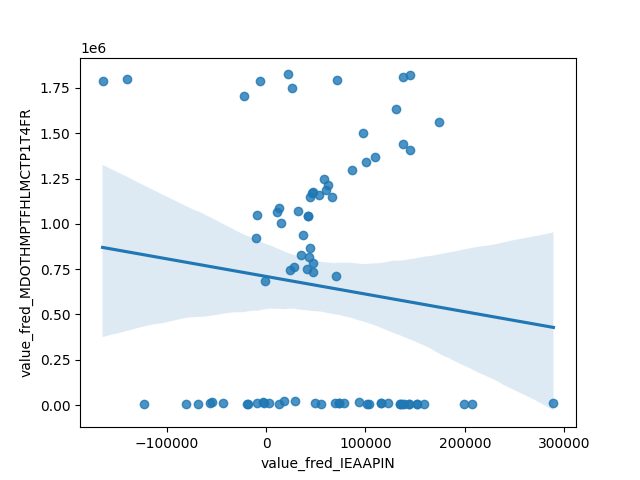
\includegraphics[scale = 0.9]{plots/plot_2026-11-16.png}
\caption{Raw Regression Plot for 2026-11-16}
\end{figure}
\newpage
\subsection{Detrended Regression}
\noindent Regresses the residuals of each series after removing its own linear time trend, so a shared trend can no longer drive the result on its own. A relationship that stays significant here is better evidence of a genuine link between the two series.

\begin{center}
\begin{tabular}{lclc}
\toprule
\textbf{Dep. Variable:}                  & value\_fred\_MDOTHMPTFHLMCTP1T4FR\_detrended & \textbf{  R-squared:         } &     0.001   \\
\textbf{Model:}                          &                     OLS                      & \textbf{  Adj. R-squared:    } &    -0.012   \\
\textbf{Method:}                         &                Least Squares                 & \textbf{  F-statistic:       } &   0.05663   \\
\textbf{Date:}                           &               Mon, 16 Nov 2026               & \textbf{  Prob (F-statistic):} &    0.812    \\
\textbf{Time:}                           &                   21:19:15                   & \textbf{  Log-Likelihood:    } &   -1208.5   \\
\textbf{No. Observations:}               &                        83                    & \textbf{  AIC:               } &     2421.   \\
\textbf{Df Residuals:}                   &                        81                    & \textbf{  BIC:               } &     2426.   \\
\textbf{Df Model:}                       &                         1                    & \textbf{                     } &             \\
\textbf{Covariance Type:}                &                  nonrobust                   & \textbf{                     } &             \\
\bottomrule
\end{tabular}
\begin{tabular}{lcccccc}
                                         & \textbf{coef} & \textbf{std err} & \textbf{t} & \textbf{P$> |$t$|$} & \textbf{[0.025} & \textbf{0.975]}  \\
\midrule
\textbf{const}                           &    4.651e-08  &     5.66e+04     &  8.22e-13  &         1.000        &    -1.13e+05    &     1.13e+05     \\
\textbf{value\_fred\_IEAAPIN\_detrended} &      -0.1765  &        0.742     &    -0.238  &         0.812        &       -1.653    &        1.300     \\
\bottomrule
\end{tabular}
\begin{tabular}{lclc}
\textbf{Omnibus:}       & 11.328 & \textbf{  Durbin-Watson:     } &    0.154  \\
\textbf{Prob(Omnibus):} &  0.003 & \textbf{  Jarque-Bera (JB):  } &   12.707  \\
\textbf{Skew:}          &  0.958 & \textbf{  Prob(JB):          } &  0.00174  \\
\textbf{Kurtosis:}      &  2.964 & \textbf{  Cond. No.          } & 7.63e+04  \\
\bottomrule
\end{tabular}
%\caption{OLS Regression Results}
\end{center}

Notes: \newline
 [1] Standard Errors assume that the covariance matrix of the errors is correctly specified. \newline
 [2] The condition number is large, 7.63e+04. This might indicate that there are \newline
 strong multicollinearity or other numerical problems.

\begin{figure}
\centering
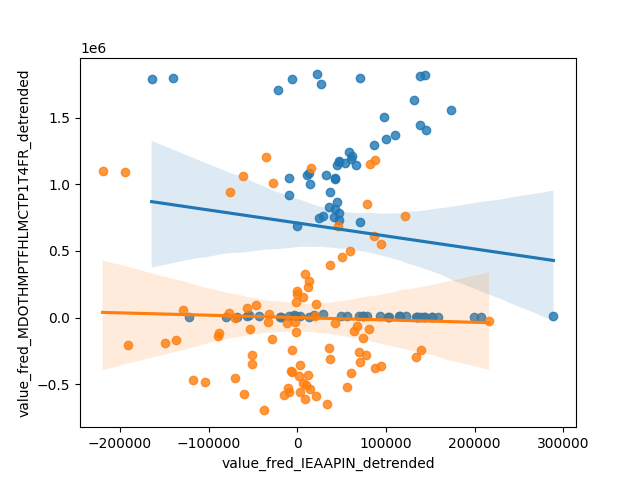
\includegraphics[scale = 0.9]{plots/plot_2026-11-16_detrended.png}
\caption{Detrended Regression Plot for 2026-11-16}
\end{figure}
\newpage
